\chapter{Collaborative Robotics}
\label{chp:2-collab-robots}

\par In this chapter, we explore the theoretical background of this work, as well as some related research done in this field. We start by giving some historical context to see when and why collaborative robots started to emerge. Then, we define the field of \ac{hrc} detailing all of its subfields and characteristics. Afterwards, we outline the current technological trends used to develop such systems and give a thorough description of the \ac{ur10e} system. Finally, we give light to several research efforts performed not only in the general field of \ac{hrc}, but also in specific problems directly correlated to this work.





\section{History}

% READ Springer Handbook of Robotics - Industrial Robots, p. 1385

% Industrial robots role in industry
\par Since the 1970s, industrial robots and manipulators have been part of production lines in many sectors of the industry. The main reason is that they can complete certain tasks faster and more efficiently than humans, since they are built with performance and precision in mind. Furthermore, a lot of manufacturing processes rely on repetitive and laborious tasks that for a human worker can become tedious and exhausting. According to the International Federation of Robotics\footnote{https://ifr.org/}, in the year 2020 there were an estimated 2.7 million industrial robots in operation worldwide \cite{wr.report.2020}.

% Need of collaboration between human and robot
\par This level of automation guarantees uninterrupted and efficient productivity in assembly lines, since robots do not take breaks or get tired, but at the same time they limit its flexibility and adaptability. When a manufacturing process, typically of customized products with smaller lot sizes, prioritizes flexibility and changeability over automation, these machines are useless and there is a need to involve a human worker in the process. An industrial robot is usually hard coded to do one task at a time, has limited abilities for handling complex or limp objects and cannot make decisions, therefore the close linkage of human and robot in these scenarios should result in the best of both sides. This collaborative approach can have several advantages compared to full automation, particularly when a robot can be guided by a human and simultaneously provide power assistance to him \cite{coop.assembly}.

% Reasons for the existence of collaborative robots
\par Traditional industrial robots have heavy structures with fixed installations, only interact with humans during programming and are otherwise separated from them through perimeter safeguarding, stopping their motion if any obstacle breaches it. These characteristics prevent them to be used in collaboration or even coexist with human workers. Given these restrictions and needs from the industry, came the concept of \ac{cobot}, firstly coined in 1996 by J. Edward Colgate and Michael Peshkin \cite{cobot.old} as '\textit{a robotic device which manipulates objects in collaboration with a human operator'}. In their work, it was a simple device with a single joint that assisted the human operator by setting up virtual surfaces which could be used to constrain and guide motion.

% Nowadays cobots do exist
\par Years later, companies like KUKA and \ac{ur} made commercially available the first industry ready cobots, denoted as industrial collaborative robots. They were light-weight, flexibly relocated and easy to teach and program, even by non-experts. Most importantly, they were equipped with power, force and speed sensors and limiters, allowing safe execution of tasks near humans, therefore allowing a shared collaborative environment. Nowadays, cobots have evolved in such a way that they are replacing industrial robots in assembly lines, or from another perspective, industrial robots are being designed with collaboration in mind.

% TODO Explain the industry need for Human Robot Collaboration - Industry 5.0

% READ Industry 5.0
% https://ec.europa.eu/info/publications/industry-50_en
% https://www.mastercontrol.com/gxp-lifeline/3-things-you-need-to-know-about-industry-5.0/
% https://medium.com/@marcellvollmer/what-is-industry-5-0-a363041a6f0a
% https://www.i-scoop.eu/industry-4-0/industry-5-0/

% TODO This leads to the emergence of Human Robot Collaboration





\section{Human Robot Collaboration}

% Explain Human Robot Collaboration
\par \ac{hrc} is a subsection of the general field of study called \ac{hri} which according to research \cite{hri.1, hri.2} is defined as '\textit{a general term for all form of interaction between humans and robots}' or '\textit{the process of conveying human intentions and interpreting task descriptions into a sequence of robot motions complying with robot capabilities and working requirements}'. It is an umbrella term used to describe a multidisciplinary field that includes knowledge and understanding from human-computer interaction, robotics, artificial intelligence, design and psychology. 

% FIXME There are many categorizations and views of HRI and HRC (cite many sources) but a general consensus revolving this subject...

% Criteria used in order to classify Human Robot Collaboration
\noindent \ac{hri} can be divided in several sub-categories based on the following four criteria \cite{paper.review.1, paper.review.2}:

\begin{itemize}
    \item \textbf{Workspace: }It is the overlapping space in the working range of human and robot;
    \item \textbf{Working Time: }The time the participants are working inside the shared workspace;
    \item \textbf{Aim: }The objective, focus and goal of each participant regarding the task at hand;
    \item \textbf{Contact: }Meaning intentional physical contact between the participants;
\end{itemize}

% Classify HRC based on the previous criteria
\noindent Using these four criteria, \ac{hri} can be divided in:

\begin{itemize}
    \item \textbf{Human-Robot Coexistence} (workspace and working time): Defined by the capability of simultaneously sharing the workspace between humans and robots, but operating in dissimilar tasks and not interacting with each other. They do not have a common goal and do not share contact therefore do not need to be synchronized. Robot abilities often rely only on collision avoidance.
    \item \textbf{Human-Robot Cooperation} (workspace, working time and aim): It is an upgrade over the previous category. Now humans and robots also share the same purpose in the given task. Cooperation also requires synchronization, which means that either exists a common language of communication, through instructions, gestures or voice, or machine vision is used for the robot to know when it is its time to act.
    \item \textbf{Human-Robot Collaboration} (all four criteria): The final stage of \ac{hri}, where humans and robots, who simultaneously share the same workspace, work together to perform a complex task interacting physically with one another. With \ac{ft} sensing hardware a robot can interpret human motion and intention, and react accordingly. 
\end{itemize}

% TODO Add a final remark on HRC
%  Human–robot collaboration allows the combination of
%  typical strengths of robots with some of the numerous 
%  strengths of humans. Typical strengths of industrial
%  robots are high stamina, high payload capacity, precision, 
%  and repeatability. Strengths of human workers
%  that are unmatched by any machinery comprise flexibility 
%  for new production tasks, creative problem-solving
%  skills, and the ability to react to unforeseen situations.

\par With HRC defined and identified inside the broader field of \ac{hri}, some of its requirements and characteristics are going to be drawn in order to proceed with a full understanding of its context.



\subsection{Hardware and Design}

% Cobot design is a general problem in the robotics field
\par The design and composition of a cobotic system can be one of the most challenging problems in this field \cite{handbook, cobot.design}. Industrial cobots generally operate in complex working conditions and must be able to carry motion effectively, sometimes in crowded environments, while facing unexpected events such as the arrival of a human operator. This is one of the reasons that cobots are usually designed with 6 to 7 \ac{dof}. Another is that an higher number of \ac{dof} provides the cobot with increased flexibility and dexterity in complex manipulation tasks.

% Cobot hardware characteristics
\par Because cobots are meant to work alongside humans, reduced weight of the moving parts is one of the main factors in cobot design \cite{cobot.light}. Even so, in environments where collisions are inevitable, the risk of interaction with cobots can be reduced due to their increased sensorial apparatus \cite{cobot.sensor}, such as the use of proximity-sensitive skins or \ac{ft} sensors to detect collisions, the increased energy absorbing properties of protective layers, the limits on robot velocity and maximum strength and force, and in some scenarios the placement of airbags around the robot \cite{cobot.airbag}.

\par According to recent reviews \cite{paper.review.1, paper.review.2}, research is still being develop on numerous different ways to improve the design of cobots in order to make them reliable, dependable and most importantly safer.

% TODO Outline robotic cells



\subsection{Safety}

% READ Design Considerations for Safe Human-robot Collaborative Workplace, 2015

% Safety standards and requirements for industrial robots
\par The general design and composition of a cobot has been shown, but is not enough to guarantee safe \ac{hrc}. According to \acs{iso} 10218:2011 \cite{iso.10218.1, iso.10218.2}, and later more widely explained in \acs{isots} 15066:2016 \cite{iso.15066}, specific requirements for cobotic systems need to be met for them to be considered safe. These standards define four classes of safety requirements for industrial robots in collaborative environments:

\begin{itemize}
    \item \textbf{Safety-rated monitored stop: }The robot is stopped upon access of the human to the collaborative workspace. Most robot manufacturers offer a safety controller that assures the standstill of the robot. The robot can then resume the task once the human has left the collaborative workspace. This mode is mostly used when the cobot works alone, but occasionally a human operator can enter its workspace. In a broader view, the robot does not move while the human is present.
    \item \textbf{Hand-guiding: }The human uses a hand-operated device, usually located at the \ac{eef} of the robot, to transmit motion commands to the robot system. This type of operation implies a direct physical interaction with the robot, where the human must have full control over its movement. The position of the human within the collaborative workspace must be defined and a safety controller for delimiting the robot speed is required. Graphic support through icons or \acs{3d} simulation is helpful for intuitive programming of the robot.
    \item \textbf{Speed and separation monitoring: }There is constant monitoring of the relative speed and distance between robot and human. The robot must maintain a minimum safe distance and speed to the human in order to be able to stop any dangerous motion if contact with the human is imminent. When the separation distance decreases to a value below the minimum, the robot stops. When the human moves away from the robot, the robot can resume motion automatically. External vision sensor data might be needed to achieve this level of monitoring since few manufacturers equip cobots with such capabilities. 
    \item \textbf{Power and force limiting: }The robot system should be designed to sufficiently reduce risk to a human by allowing direct, physical interaction without an additional safety controller. This is done through the design of the robot system by limiting collision forces so that in the event of a contact between the humans and the robot, biomechanical tolerance limits are not exceeded.
\end{itemize}

\par A traditional industrial robot can be adapted to meet this collaborative modes and requirements, however it would need additional safety devices such as laser sensors, vision systems, or controller modifications. For this reason, a commercial cobot that has this features built-in requires no further hardware costs and can be a more attractive solution.



\subsection{Programming}

% Traditional industrial robots are hard to program
\par Industrial robots have the job of carrying out pre-programmed, repetitious tasks in order to promote productivity and efficiency. Their software platform is responsible for enabling \ac{hri} and conveying human intention on how certain tasks should be executed. Intuitive robot programming is an important issue that \ac{hri} deals with, since traditional approaches are either unintuitive or time-consuming. In the early days of industrial automation, robots could only be programmed by experts in actuators, controllers and hardware programming.
% Collaborative robots come with teach pendants
Nowadays, most industrial robots are shipped with teach pendants. These are handheld devices containing buttons, switches and, in some cases, a touchscreen. They are currently the most common programming method as they require little to no training in robotics or programming in general, they display the robots commands in a nontechnical fashion and allow for online editing of such commands. They also allow for walk-through programming where an operator physically moves the robot through a desired task. Although these methods seem intuitive and easy to learn, they are only applicable for certain groups of tasks since they have low accuracy requirements, and for complex tasks can become cumbersome to use.
% A good technique for robot programming is the use of robotic skills
\par Finding accurate, intuitive and efficient ways for robot programming is also a problem for \ac{hri}. One possible and currently established technique is the generation of robotic skills, which are pre-programmed software packages that only need to be parametrized by the user. A recent study \cite{cobot.skill} has introduced a software architecture combining generation of robotic skills, named action blocks, that also allowed for process control, and a set of strategies and approaches for a fast and intuitive parametrization process.
% Various ways for robot programming
\par Further research in this area is constantly looking for better user interfaces for robot programming \cite{paper.review.1, cobot.reality}. A few examples are:

\begin{itemize}
    \item \textbf{Virtual Reality: }Where tasks are completed intuitively as if the human is present at the remote working environment. It guarantees safe programming and is flexible on the level of workspace constraints or task complexity that may exist. The main problem is that it requires previous knowledge of the working areas to construct the virtual environment, and is not suitable for loosely structured working conditions where there may be constant changes to the environment.
    \item \textbf{Augmented Reality: }Where virtual elements, mainly computer-generated graphics, are projected into the real world so that the user can perceive certain elements of robot programming in real-time. Such elements might include objects, robot motions and trajectories, and  simulated collisions with the real environment. This technique can also help operators determine the best location for the robot before final installation.
    \item \textbf{Program by Demonstration: }Where a human performs a task manually and in parallel, the robot is observing, following and learning the task in real-time. It allows any user to program a robot by just giving a demonstration of the sequence of operations to be carried out and shifts the burden of robot programming from robot experts to task experts. It also makes possible to program more than one robot simultaneously. A significant problem with this approach is that jerks and inaccuracies in human demonstrations can lead to unsatisfactory execution of tasks by the robot that is learning them.
\end{itemize}

% Final remark in robot programming
\par Other approaches on robot programming are also moving forward towards multimodal interfaces with the inclusion of gestures, voice, eye gaze and facial expressions serving as high-level inputs to control and program the robotic system.

% TODO Add section on Collaborative Tasks
% mashable,  e-series brochure, universal robots website
% - https://www.universal-robots.com/media/1802432/e-series-brochure.pdf





% TODO Change the name to Technologies and Background, or similar
\section{Predominant Technologies}

% TODO Subsection on high level robot control with behavioral trees and ros_smach

% Section intro
\par In a cobotic system, the interaction between the robot, the user, the external sensors and software modules usually rely on several different technologies, all working together to provide a seamless and efficient experience. Below, divided in various categories is explained which technologies are going to be used in this work and why. 



\subsection{Robotics Middleware}

% Middleware definition
\par A middleware is a piece of software that enables cohesive, structured communication between different software modules. It is informally described as "software glue". It has been shown that a cobotic system is comprised of different components, that usually are handled by different software modules, known as their drivers. These modules may be written in different programming languages and implement different communication protocols. As such, the job of a middleware is to hide the obvious heterogeneity resultant of a system with these characteristics, and provide functions and services that not only enhance the communication between the entities, but also serve as a flexible, interoperable and central repository of information shared by them.
% Intro to ROS
\par The \ac{ros} \footnote{https://www.ros.org/} \cite{ros} is an open-source robotics middleware. With over 3.000 packages in its ecosystem, it is also described as a flexible framework for writing robot software, that comprises a plethora of tools, libraries, and conventions that aim to simplify the task of creating complex and robust robot behavior across a wide variety of robotic platforms. A key component of a cobotic system is its communication infrastructure and \ac{ros}, at its lowest level, offers a message passing interface that provides inter-process communication and implements a publisher/subscriber communication model. Each component that performs a certain task is called a \ac{ros} node, and multiple nodes communicate between them by exchanging \ac{ros} messages through \ac{ros} topics. These provide an asynchronous means of communication, since any node can publish or subscribe to any topic at any time, provided it respects its message type. For synchronous communication, \ac{ros} offers services which can be seen as remote procedure calls that provide request/response interactions between nodes. The middleware part of \ac{ros} also provides a global key-value server where nodes can set and get configuration parameters.
% Robotic features of ROS
\par When it comes to robot specific features, \ac{ros} provides libraries that help their integration  in its ecosystem through collections of software drivers, that abstracts both the low-level control of hardware components, and the treatment of information generated by sensors and other peripherals. A crucial example of such functionality is the Robot Geometry Library\footnote{http://wiki.ros.org/tf} which helps keeping track of where different parts of the robot are with respect to each other and the world. Therefore, it allows the user to define both static transforms, such as a camera that is fixed somewhere in the world, and dynamic transforms, such as the pose of the \ac{eef} in a manipulator. This way, any positional data can be easily transformed between any pair of coordinate frames in the world.
% Extra features of ROS
\par Other features that enhance the development of such systems include RViz\footnote{http://wiki.ros.org/rviz} which provides \acs{3d} visualization of robot description models, transforms and many sensor data such as point clouds; an extensive library of built-in plugins based on rqt\footnote{http://wiki.ros.org/rqt}, which is a Qt-based framework for developing graphical interfaces that easily integrates with the \ac{ros} ecosystem; a set of command-line tools that allow the user to fully control all \ac{ros} core functionality without a \ac{gui}, useful for controlling the cobotic system remotely.

% TODO Talk about NVIDIA Isaac and ROS 2



\subsection{Universal Robots UR10e}
\label{ssec:ur10e}

% The work will be implemented on a UR10e
\par Although the techniques developed in this dissertation are generic, the cobot with which this work will be implemented is an \ac{ur10e}. It is a 6 \ac{dof} collaborative industrial robot equipped with a \ac{ft} sensor in its \ac{eef}. A visual description of its configuration is show in \autoref{fig:ur10e}, detailed technical specifications are shown in \autoref{tbl:ur10e-specs}, and the various ways that it can be controlled will be explained below, as well as the chosen method and why.

\begin{figure}[h]
    \centering
    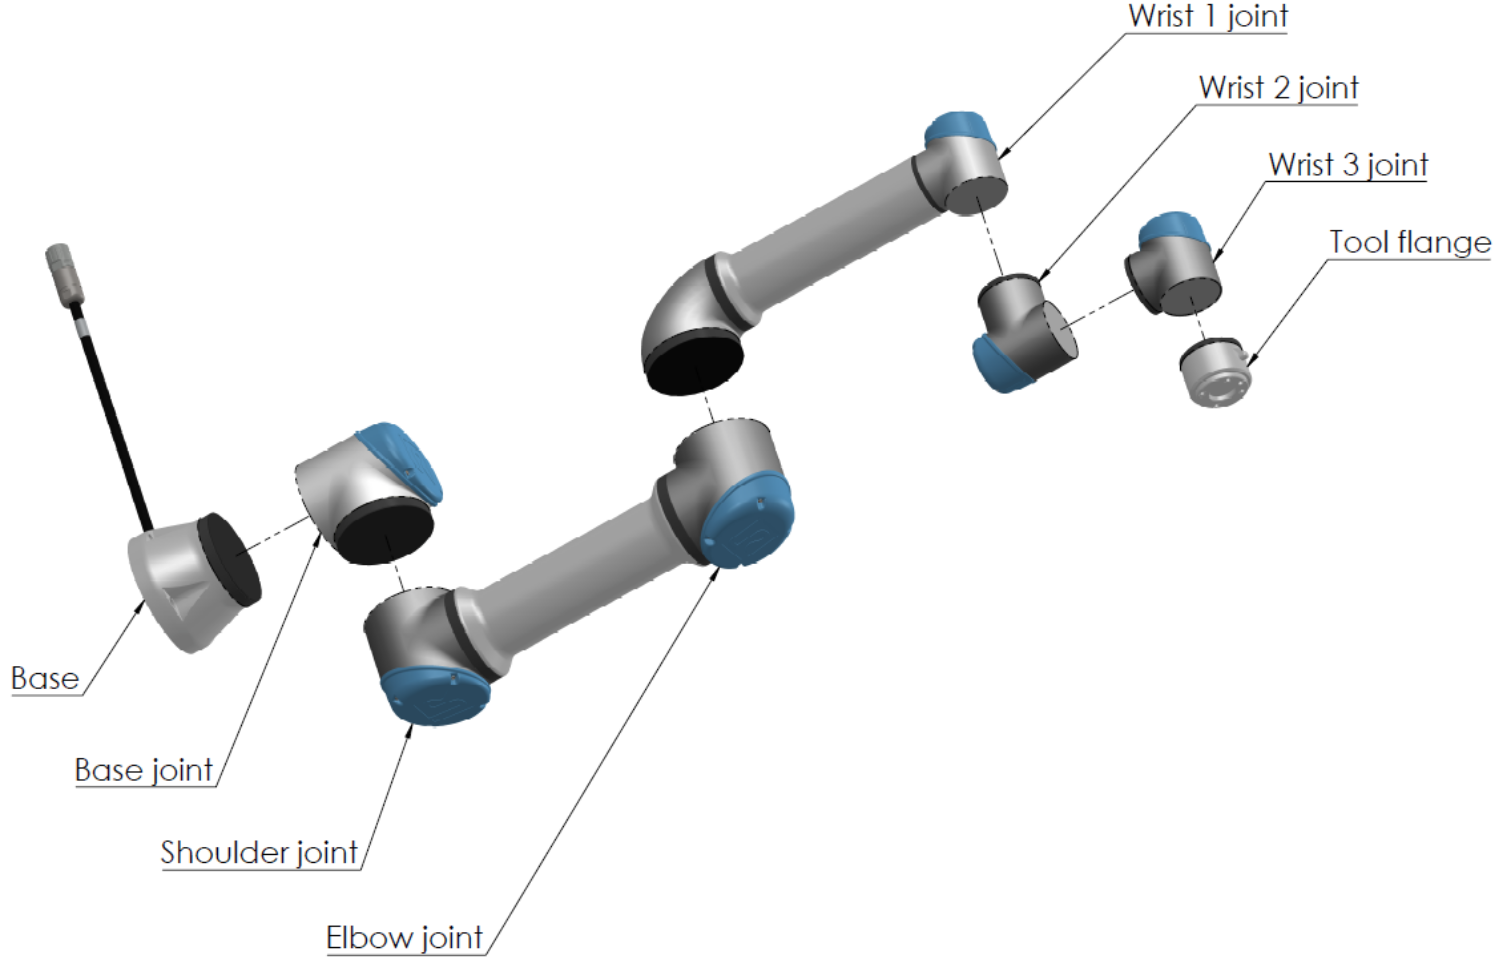
\includegraphics[width=0.8\linewidth]{figs/chp2/ur10e.png}
    \caption{Joint configuration of the \ac{ur10e}}
    \label{fig:ur10e}
\end{figure}

% UR10e technical specifications table
\begin{table}[htp]
    \centering
    \begin{tabular}{|l|l|lllll}
    \cline{1-2}
    \textbf{\ac{ur10e}} & \textbf{Value} &  &  &  &  &  \\ \cline{1-2}
    Reach & 1300 mm &  &  &  &  &  \\ \cline{1-2} \cline{5-7} 
    Payload & 10 Kg &  & \multicolumn{1}{l|}{} & \multicolumn{1}{l|}{\textbf{\ac{ft} Sensor}} & \multicolumn{1}{l|}{\textbf{Force}} & \multicolumn{1}{l|}{\textbf{Torque}} \\ \cline{1-2} \cline{5-7} 
    \ac{dof} & 6 rotating joints &  & \multicolumn{1}{l|}{} & \multicolumn{1}{l|}{Range} & \multicolumn{1}{l|}{100 N} & \multicolumn{1}{l|}{10 Nm} \\ \cline{1-2} \cline{5-7} 
    Pose Repeatability & +/- 0.05 mm &  & \multicolumn{1}{l|}{} & \multicolumn{1}{l|}{Resolution} & \multicolumn{1}{l|}{2.0 N} & \multicolumn{1}{l|}{0.02 Nm} \\ \cline{1-2} \cline{5-7} 
    Joint Working Range & ± 360 ° &  & \multicolumn{1}{l|}{} & \multicolumn{1}{l|}{Accuracy} & \multicolumn{1}{l|}{5.5 N} & \multicolumn{1}{l|}{0.60 Nm} \\ \cline{1-2} \cline{5-7} 
    Joint Maximum Speed & ± 120 °/Sec. &  &  &  &  &  \\ \cline{1-2}
    Typical \ac{eef} Speed & 1 m/Sec. &  &  &  &  &  \\ \cline{1-2}
    Footprint & 190 mm &  &  &  &  &  \\ \cline{1-2}
    Weight & 33.5 Kg &  &  &  &  &  \\ \cline{1-2}
    \end{tabular}
    \caption{\acl{ur10e} technical specifications}
    \label{tbl:ur10e-specs}
\end{table}

\subsubsection{Teach Pendant}

\par The \ac{ur} teach pendant is a handheld wired device with a 12 inch touchscreen display that allows the user to fully configure and control the \ac{ur10e}. It does so using the Polyscope \cite{ur10e.manual}, a graphical user interface that operates the robot arm and control box, creates and executes programs. It terms of operational modes it allows compliant motion with the Freedrive mode, manual motion with arrow buttons and sliders, and automatic motion with the creation of programs using its built-in programming environment, which is seen as a programming tree where the user adds programming nodes. These nodes can be commands telling the robot what to do or generic programming statements (if, loop, event, etc.). Polyscope allows people with little programming experience to program the robot and for most tasks it is done entirely using the touch panel without typing any cryptic commands. Given its simplicity, it is not ideal for complex tasks, or if the user needs low-level control or sensor information access. Besides the programming features, the teach pendant is also equipped with a button in the back that enables the Freedrive mode and an emergency stop red button in the front.

\subsubsection{URScript}

\par Parallel to the Polyscope interface, \ac{ur} also provides a script level way of controlling its robots through their own programming language, called URScript \cite{urscript.manual}. This language includes variables, types, flow control statements and functions that monitor and control both \acs{io} and robot movements. Inside the Control Box of the robot there is a low-level controller called URControl. Programming a robot at the script level is done by writing a client application and connecting to URControl using a \acs{tcp}/\acs{ip} socket. When a connection has been established URScript programs are sent on the socket. Compared to the Polyscope interface, URScript gives the user more control over the structure of the programs and makes it easier for an experienced user to take full advantage of the robot. One downside to this approach is the user that is sending commands externally has no access to the current state of the program, since once the program is sent, it is executed immediately without feedback. The only way the user can access the state of the robot is by connecting to another one of the available client interfaces\footnote{https://www.universal-robots.com/articles/ur/interface-communication/overview-of-client-interfaces/} that publish robot information at a fixed rate interval.

\subsubsection{Universal Robots \acs{rtde} Interface}

\par The \ac{rtde}\footnote{https://www.universal-robots.com/articles/ur/interface-communication/real-time-data-exchange-rtde-guide/} interface provides a way to synchronize an external application with the \ac{ur} controller over a standard \acs{tcp}/\acs{ip} connection. This functionality is split in two stages, a setup procedure and a synchronization loop. In the setup procedure, the external application will become a client of the \ac{ur} controller, over the \ac{rtde} interface by sending a recipe. This recipe should contain a setup list of named input and output fields that should be exchanged in the synchronization loop. When this loop is started, the \ac{rtde} interface sends data to the client in the same order that the client requested. On an e-Series \ac{ur} cobot, such as the \ac{ur10e} the \ac{rtde} interface generates output messages at 500Hz. 
\par Researchers at University of Southern Denmark have developed a C++/Python library for controlling and receiving data from a \ac{ur} robot using the \ac{rtde} interface, called ur\_rtde\footnote{https://gitlab.com/sdurobotics/ur\_rtde}. It makes available three distinct interfaces: 

\begin{itemize}
    \item \textbf{\ac{rtde} Control Interface: }Primarily used for moving the robot and utility functions. It requires a control script to be running on the robot, which is uploaded automatically.
    \item \textbf{\ac{rtde} Receive Interface: }Used for receiving data from the robot.
    \item \textbf{\ac{rtde} \acs{io} Interface: }Used for setting digital/analog \acs{io} and adjusting the speed slider of the robot.
\end{itemize}

\noindent The Control Interface allows for non-blocking commands making the flow of the external program able to continue while the robot is moving. The separation of Control and \acs{io} in different interfaces also allows to change the speed of the robot while it is moving. 
\par Although it takes programming knowledge and skills, from all the available ways to control a \ac{ur} cobot, the use of the \ac{rtde} interface has proved to be the most advantageous one.

% TODO Explain better the messages exchanged

\subsubsection{Universal Robots \ac{ros} Driver}

\par The goal of this driver is to provide a stable and sustainable interface between \ac{ur} robots and \ac{ros}, that both enhances the control of the robots using \ac{ros} paradigms such as its controller interface, and makes available to the \ac{ros} environment all data regarding the robot. By using \ac{ros} compatible manipulators, perception sensors, peripherals and motion planners the user makes sure all components speak the same language and interoperate regardless of \acs{oem} brands or communication protocols. Further implementation details can be found in~\cite{ur.ros.driver}.
\par In terms of features, this driver uses the \ac{rtde} interface for communication; uses the speed-scaling of the robot for slowing down trajectory execution accordingly; serves as a replacement for the teach pendant since it offers \ac{ros} services for most of its interactions, such as start, stop and even recover the robot from safety events; uses on-the-robot interpolation for joint-based trajectories, which helps if the application can not meet the real-time requirements of the \ac{rtde} interface; and many more, extensively documented in the \ac{ur} github repository\footnote{https://github.com/UniversalRobots/Universal\_Robots\_ROS\_Driver}.
\par This driver is currently being updated to both include with new functionality and support new \ac{ur} software updates. Recent important features include joint velocity-based control that lets the user directly control the speed of each individual joint, which is very helpful for visual servoing, real-time motion planning or other kinds of control that require speed control rather than position control, and cartesian position-based and twist-based control that lets the user execute trajectories along cartesian paths.
\par The \ac{ur} \ac{ros} Driver will be the chosen method of interfacing with the \ac{ur10e} for the amount of extra functionality it provides and the overall advantages of developing software in the \ac{ros} ecosystem.



\subsection{Motion Planning}

% READ Springer Handbook of Robotics - Kinematics, p. 11

\par Motion planning is a computational problem with the objective of planning motions for complex bodies from a start to a goal position. It breaks down a desired movement task into discrete motions that satisfy movement constraints while avoiding collision with known obstacles.
\par The MoveIt Motion Planning Framework \cite{moveit.paper, moveit.online} is an easy-to-use open source robotics manipulation platform for developing commercial applications, prototyping designs, and benchmarking algorithms. Its main strength is the ability to generate high \ac{dof} trajectories trough cluttered environments and avoid local minimums. It also provides robot description and kinematics implementations for multiple robot manipulators. One of its features that is relevant to this Dissertation is the implementation of the \ac{ompl}, which aggregates many state of the art motion planning algorithms. One of which is the \ac{rrt} Connect planner which will be the default motion planner used in this work.
\par In this work, MoveIt will be used mostly for offline position-based trajectory planning. One of the objectives is to control the robot in real-time, with velocity-based commands sent at high frequency. As of writing, current MoveIt releases do not support such features, having only plans to implement them in future versions. Further details on the solution of this problem will be presented in \autoref{section:pf-method}.

% TODO Robot Kinematics, APF, and general improvements



\subsection{Perception}

\par To fully achieve collaboration in a shared environment, the cobot must be able to perceive its surroundings. Between the various ways to give the cobot this ability, the majority of them rely on external sensors, such as stereo or depth cameras, and lidar sensors. All of them give the system a \acs{3d} representation of their field of view through the generation of point clouds.
% PCL
\par The \ac{pcl} \cite{pcl} is a standalone, large scale, open project for \acs{2d}/\acs{3d} image and point cloud processing. It is split into a series of modular libraries ranging from filters, recognition, segmentation and visualization. It will be extensively used in this work to achieve the obstacle avoidance task which will be further explained in \autoref{section:obstacle-detection}.
% Calibration
\par To be able to identify obstacles in relation to the cobot, a process known as camera extrinsic calibration needs to be performed. It consists on identifying in the cartesian space where the perception sensor is, in relation to the robot. Only this way, can the obstacles identified by the sensor be spatially placed in the shared environment. The \textit{easy\_handeye} \ac{ros} package\footnote{https://github.com/IFL-CAMP/easy\_handeye} is an implementation of the highly cited work of R. Y. Tsai and R. K. Lenz \cite{handeye} where a fully autonomous and efficient technique for \acs{3d} robotics hand eye calibration is developed. In the scenario that will be implemented in this Dissertation, where the sensor is fixed in the world, this package it able to obtain a static transform from the world frame to the sensor, by capturing images of a fiducial marker attached to the \ac{eef} of the robot. Then using the Tsai-Lenz algorithm implemented in the OpenCV library computes the result and stores it in the \ac{ros} environment.

% READ A General Approach to Hand–Eye Calibration Through the Optimization of Atomic Transformations





% FIXME Change the name to Similar Research, ou similar
\section{Existing approaches}

% There are no full features integrated, close, solutions
\par In the topic of collaborative tasks between a human and a cobot, there is no record of  commercially available, full-featured frameworks or systems, that could allow the accomplishment of the objectives proposed in this dissertation. Even though manufacturers ship their cobots and accessories with extensible and flexible software, that allow the creation of such tasks, there is much work left for the user to design, program and implement the system architectures that aggregate the collaborative tasks and deliver a cohesive, seamless experience. Furthermore, there is no limit on the amount of collaboration that can exist, or on how the available tools can be used together in their final working environments.
% There are many efforts from research
Despite these facts, extensive research efforts have, and are currently being made \cite{paper.review.1, paper.review.2} to enhance this field with structured architectures and frameworks that seamlessly allow multifaceted collaboration between human and cobot. This section serves as a survey on such proposals, and will firstly enumerate and detail general approaches to \ac{hrc} and collaborative tasks. Then, it will shift to other solutions that directly correlate to specific problems faced in this Dissertation, and that also served as inspiration to the solutions implemented. 



% TODO Review section with newer papers
\subsection{Proposals on \acs{hrc} and Collaborative Tasks}

% READ Trends of Human-Robot Collaboration in Industry Contexts: Handover, Learning, and Metrics
% READ Review of Interfaces for Industrial Human-Robot Interaction

\par The work in \cite{colab.framework} proposes a collaborative framework for robotic task specification, where the authors start by stating that the lack of effective sensing and task variability creates too much uncertainty to reliably hard-code a robotic cell. The developed framework blends automated task specification with the experience and cognition of a human operator to provide a more accurate task specification. This work was implemented with \ac{ros} and was mainly focused on surface finishing tasks.

\par The authors in \cite{colab.cell} deal with the problem of developing a collaborative coating cell. They start by teaching the robot its trajectory with a programming by demonstration technique, using a multicolored \acs{led} marker attached to the coating tool. Then, a \acs{3d} perception system was developed to perform initial point cloud alignment and 6 \ac{dof} pose estimation. Finally, to promote safe \ac{hrc}, a zone monitoring system was employed to track the position of the operator inside the cell.

\par A coordination system for assembly tasks where HRC is required was presented in \cite{colab.assembly}, where the authors developed a \ac{ros} based framework that intertwined a sequence of tasks modeled in a neutral \acs{xml} format language, with the ability for human and a robot to coexist in a fenceless cell, where safety was guaranteed by a \acs{3d} industrial safety camera.

\par Regarding a polishing task, authors in \cite{colab.polishing} proposed and demonstrated the use of a robotic manipulator with an \ac{ft} sensor in its \ac{eef}, whose task was to keep a workpiece in a prescribed sequence of poses while a human operator, equipped with an abrasive tool, proceeded to polish it. They also allowed the operator to change the orientation of the workpiece mounted on the robot, by physically pushing or pulling the robot body. They achieved this behavior with a control algorithm that was able to distinguish polishing forces applied at the \ac{eef} level, from the external torques acting on the robot joints due to the intentional physical interaction engaged by the human.

\par Research in \cite{colab.skill} resulted in the development of a cobotic framework applied to solve a screwing task in collaboration with a human operator, using a skill-based approach. The \ac{ros}-based system used a software called Skill Based System, which treats tasks as a set of skills, which then are composed of sequences of motion primitives. The human operator was then able to execute programmed tasks or create new ones using the available skills.

\par A framework for the execution of collaborative tasks in hybrid assembly cells was developed in \cite{colab.assembly.cell}, where the focus was given to the human-robot coexistence for the execution of sequential tasks, in order for the automation level in assembly lines to be increased. Even though not strictly dealing with human-robot physical interaction, this work is relevant in the sense that the authors also developed a gesture based communication protocol between the human and the robot, and proved that the introduction of human-robot task allocation and execution benefitted the efficiency of the assembly process in question.

\par A system for end-user creation of robust task plans was developed in \cite{colab.costar}, where a Behavior Tree-based task editor integrates high-level information from known object segmentation, pose estimation with spatial reasoning, and robot actions to create robust task plans. The system was implemented on multiple cobots and performed a wide variety of tasks such as collaborative assembly, wire bending, sanding and polishing.

\par A multimodal \ac{hri} framework is presented in \cite{colab.multimodal} where the authors used speech, hand gesture recognition, text programming, and interaction capabilities to allow the user to intuitively program the robot and take over its control at any given time. 



\subsection{Solutions to Specific \acs{hri} Problems}

\par A method for precision \ac{hg} of a cobot at the \ac{eef} level is presented in \cite{spec.handguide}. In this work, the authors are able to obtain \ac{hgft} from the \ac{eef} \ac{ft} measurements. Then, a control scheme to govern the linear/angular motion of the \ac{eef} is described and implemented. The characteristics of the \ac{hg} task in this Dissertation has many similarities with this approach, since the former was heavily inspired by the latter.

\par The work in \cite{spec.compensation} describes a tool compensation technique to ease and simplify the process of trajectory learning in common industrial setups. It allows the user to directly use the real tool attached to the \ac{eef} while \ac{hg} the robot. It was crucial to understand the effects of coupled weight in the robot \ac{eef} and create the compensation model implemented in this Dissertation for the object manipulation task.

\par A state of the art on-line collision avoidance framework is proposed in \cite{spec.collision}, where the authors represent in space the human and the robot as capsules, and calculate their minimum distance and relative velocity. With these values, a repulsion vector is created. On the other hand, with a pre-established path generated offline, an attraction vector is computed and forces the robot into following the defined trajectory. With these two components, the implemented control algorithm is able to adjust the robots trajectory in real time, so that it is able to avoid collision with the human and simultaneously fulfill the task.

\par While studying the problem of collision prediction, the authors in \cite{spec.selfidentification} developed a method for robot self-identification based on a over-segmentation approach and the kinematic model of the robot. A similar method will be implemented in this Dissertation, since the vision system will be based on an \acs{rgbd} camera, and the points belonging to the robot must be segmented from the raw point cloud.

\par The KUKA Sunrise Toolbox \cite{spec.kuka} is a MATLAB toolbox developed to interface and control KUKA iiwa robots. It contains functionalities for networking, real-time control, point-to-point motion and physical interaction. This work heavily inspired the contributions made to the \textit{iris\_sami} \ac{ros} package and the development of the plugins \textit{rqt\_sami} and \textit{rqt\_cobot}, where similar features were developed for \ac{ur} cobots.





% TODO Add section on Discussion
% \section{Discussion}

% - Tendo em conta o que foi dito anteriormente retirar conclusões que justifiquem o trabalho que foi feito
% -   Explicar que esta tese foca-se em real time collaborative robotics e não apenas em planeamento estático com MoveIt
% - Mais uma vez, dar ênfase nas restrições que existem em software proprietário e na falta de algoritmos e metodologias abrangentes e open source para a criação de tarefas colaborativas
% - Usar o UR teach pendant como exemplo, apontar falhas e explicar como o que se segue as pode resolver
% - Bom exemplo de como fazer um capítulo destes na tese dos drones

